\documentclass[12pt]{article}

% ── Packages ────────────────────────────────────────────────────────
\usepackage[utf8]{inputenc}
\usepackage[T1]{fontenc}
\usepackage{amsmath,amssymb,amsfonts}
\usepackage{bm}
\usepackage{booktabs}
\usepackage{graphicx}
\usepackage{xcolor}
\usepackage{hyperref}
\usepackage{multirow}
\usepackage{enumitem}
\usepackage[margin=1in]{geometry}
\usepackage{natbib}
\usepackage{caption}
\usepackage{subcaption}
\usepackage{algorithm}
\usepackage{algpseudocode}

\graphicspath{{figures/}}

\hypersetup{
  colorlinks=true,
  linkcolor=blue,
  citecolor=blue,
  urlcolor=blue,
}

% ── Title ───────────────────────────────────────────────────────────
\title{\vspace{-2em}\textbf{Causal-LeWM: End-to-End Causal Object-Centric World Models\\ via Joint-Embedding Prediction with Structured Regularization}\vspace{-1em}}

\author{
  % Author list to be filled in
}

\date{\today}

\begin{document}
\maketitle

\begin{abstract}
Object-centric world models that induce causal structure through latent interventions (e.g., C-JEPA) currently depend on frozen pretrained encoders, while end-to-end JEPA training with Sketched Isotropic Gaussian Regularization (SIGReg) has been demonstrated only on unstructured global embeddings. We propose \textbf{Causal-LeWM}, which combines C-JEPA's object-level masking with SIGReg-based regularization to train the full encoder--slot-attention--predictor stack from pixels on Push-T manipulation. The central obstacle is a \emph{dual collapse} problem: JEPA representational collapse and slot-attention collapse arise simultaneously, and we show empirically that they have opposite signatures and require complementary, non-substitutable countermeasures --- per-slot SIGReg and a variance hinge alone yield decorrelated \emph{noise} slots; feature reconstruction alone yields a degenerate one-slot autoencoder; only their combination with a within-frame decorrelation loss and stable learned slot anchors produces slots that are simultaneously distinct, grounded, and predictable. Beyond collapse, we identify \emph{temporal slot identity} as the dominant factor in predictive quality: in a controlled three-seed ablation, SAVi-style slot propagation reduces normalized prediction error from $0.790 \pm 0.014$ to $0.235 \pm 0.030$ ($3.4\times$; $\sim$21\% $\rightarrow$ $\sim$77\% of slot variance explained) with reconstruction and slot health unchanged --- the gain is purely predictive. Finally, we unfreeze the DINOv2 backbone and train fully end-to-end: training is stable (no slot or feature collapse; NMSE $0.317$ at matched steps versus $0.235 \pm 0.030$ frozen), and the finetuned model produces the qualitatively crispest object binding of all variants. Curiously, decoder-visible slot-identity stability and predictive quality dissociate: the non-propagated model keeps slot roles fixed across time yet predicts $3.4\times$ worse. In CEM-MPC planning, however, all learned policies sit at the random-action floor while a replay oracle confirms the harness is sound; we report this as a negative result and attribute it not to the world model but to an architectural mismatch between a coarse latent-space MSE cost and a high-precision ($20$\,px) control task, which scopes the contribution as representational and motivates pose-aware costs and per-step action conditioning as the path to control. Our implementation comprises $\sim$2{,}100 lines of Python, generalizing the LeWM training stack from a single [CLS] embedding to a structured $(T, N, D)$ slot tensor.
\end{abstract}

% ── 1. Introduction ─────────────────────────────────────────────────
\section{Introduction}

Learning structured world models from raw pixels has emerged as a central challenge in building agents that can reason, plan, and generalize~\citep{lecun2022}. Two recent advances bring complementary strengths to this problem, yet their combination remains unexplored.

On one side, \textbf{C-JEPA}~\citep{nam2026cjepa} extends the Joint-Embedding Predictive Architecture~\citep{assran2023ijepa} from image patches to object-centric slot representations~\citep{locatello2020slot}. By masking individual object slots and requiring the predictor to infer masked objects from visible ones, C-JEPA induces \emph{latent interventions} with counterfactual-like effects. This yields dramatic improvements: $\approx$20\% absolute gain in counterfactual reasoning on CLEVRER (68.8\% vs.\ 47.7\%) and an $8\times$ speedup in MPC planning versus patch-level world models. However, C-JEPA's object-centric encoder remains \textbf{frozen}---a pretrained DINOv2 ViT-S/14~\citep{oquab2023dinov2} serving as a fixed feature extractor. Performance is therefore ceiling-limited by the encoder's task-agnostic pretraining, and the encoder cannot adapt its object decomposition to the downstream dynamics.

On the other side, \textbf{LeWorldModel (LeWM)}~\citep{maes2026lewm} demonstrates the first JEPA that trains stably end-to-end from raw pixels. With only two loss terms---next-embedding prediction and SIGReg---LeWM eliminates the need for stop-gradients, EMA, pretrained encoders, or auxiliary supervision that plagued prior end-to-end JEPA attempts. At $\sim$15M parameters, it matches or exceeds the performance of much larger foundation-model-based world models while planning up to $48\times$ faster. Yet LeWM operates on a \textbf{single global [CLS] embedding}, discarding spatial and object-level structure entirely.

\textbf{The gap:} No existing work combines C-JEPA's object-level causal inductive bias with LeWM's end-to-end training stability. Doing so would produce a world model whose encoder learns task-adapted object representations directly from pixels, while maintaining the causal structure that object-level masking provides.

\textbf{Our contributions.} We present \textbf{Causal-LeWM} and an empirical study of its training dynamics on Push-T manipulation~\citep{chi2023diffusion}:
\begin{enumerate}[label=(\roman*)]
    \item \textbf{Architecture.} A slot-level JEPA: a ViT encoder followed by iterative slot attention produces $N$ object-centric slots per frame; a masked transformer predictor with AdaLN-zero conditioning operates over the $(T, N, D)$ slot tensor, reconstructing masked history slots and predicting future slots; a DINOSAUR-style spatial-broadcast decoder~\citep{seitzer2023dinosaur} grounds slots in encoder features.
    \item \textbf{A dissection of the dual-collapse problem.} Through a controlled ablation series we show that JEPA collapse and slot collapse have opposite metric signatures, that each regularizer removed in isolation re-opens a specific named failure mode, and that the resulting five-term objective escapes both collapse modes simultaneously at scale (\S\ref{sec:collapse}).
    \item \textbf{Temporal slot identity as the predictive bottleneck.} A controlled three-seed ablation of SAVi-style slot propagation~\citep{kipf2021savi} --- the single flag flipped, all else identical --- cuts normalized prediction error from $0.790 \pm 0.014$ to $0.235 \pm 0.030$, with no seed overlap and reconstruction/slot-health metrics unchanged across arms (\S\ref{sec:savi}).
    \item \textbf{End-to-end stability.} Unfreezing the DINOv2 backbone and training the full stack from pixels is stable under our objective: no slot collapse, no destruction of pretrained features, and the qualitatively sharpest object binding of all model variants, at a modest cost in prediction error at matched steps (\S\ref{sec:e2e}, \S\ref{sec:qual}).
    \item \textbf{A dissociation between decoder-visible slot-identity stability and prediction.} The non-propagated model assigns slot indices to scene roles \emph{more} stably over time than either SAVi variant, yet predicts $3.4\times$ worse --- evidence that what slot propagation provides to the predictor is not index--role rigidity but a usable temporal correspondence in latent space (\S\ref{sec:qual}).
\end{enumerate}

We provide a complete open-source implementation ($\sim$2{,}100 lines of Python), a planning-evaluation harness mirroring LeWM's CEM-MPC protocol, and a reproducible multi-seed experiment log.

% ── 2. Related Work ─────────────────────────────────────────────────
\section{Related Work}

\subsection{Joint-Embedding Predictive Architectures}

I-JEPA~\citep{assran2023ijepa} introduced the idea of predicting latent representations of masked target regions from a visible context region, applied to image patches within a single frame. This was extended to video sequences by V-JEPA and to object-level representations by C-JEPA~\citep{nam2026cjepa}. The key insight of C-JEPA is that masking at the \emph{object} rather than \emph{patch} level forces the predictor to model inter-object relationships, inducing a causal inductive bias without requiring explicit causal annotations. Our work builds directly on C-JEPA's predictor architecture and masking strategy but unfreezes the encoder to enable end-to-end learning.

\subsection{End-to-End World Model Training}

Training world models from pixels while maintaining representational stability is notoriously difficult. Approaches like Dreamer~\citep{hafner2023dreamerv3} and TD-MPC~\citep{hansen2022tdmpc} use reconstruction-based objectives with auxiliary losses. VICReg~\citep{bardes2022vicreg} introduced variance-invariance-covariance regularization for self-supervised learning, showing that explicit regularization can prevent collapse without contrastive negatives. LeWM~\citep{maes2026lewm} adapted this insight to JEPA training through SIGReg---a sketched Gaussian matching statistic that enforces isotropic structure on the latent distribution. LeWM reduces tunable hyperparameters from 6 to 1 (the SIGReg weight $\lambda$) while achieving competitive planning performance.

\subsection{Object-Centric Learning}

Slot Attention~\citep{locatello2020slot} introduced a simple iterative attention mechanism that competitively binds input tokens to a fixed set of slot vectors via softmax normalization over slots. SAVi~\citep{kipf2021savi} extended it to video by initializing each frame's slots from the previous frame's output, giving slots a persistent temporal identity; VideoSAUR~\citep{wu2023videosaur} and DINOSAUR~\citep{seitzer2023dinosaur} combine slot attention with self-supervised ViT features, the latter reconstructing the ViT feature map (rather than pixels) through a spatial-broadcast decoder. Prior object-centric world models either use frozen encoders (C-JEPA, SAVi) or reconstruction-based training (OCVP~\citep{villarcorrales2022ocvp}), not the combination of JEPA prediction losses with end-to-end regularization that we pursue. Our results give a precise reason SAVi-style propagation matters for world modeling: it makes the per-index prediction target well-posed (\S\ref{sec:savi}).

\subsection{Cross-Entropy Method for MPC}

The Cross-Entropy Method (CEM)~\citep{rubinstein2004cem} is a sampling-based optimizer widely used for model-predictive control with learned dynamics. At each planning step, action sequences are sampled from a Gaussian, rolled out through the learned model, scored by a cost function, and the distribution is refit to the top-$k$ elite samples. CEM was used by both C-JEPA and LeWM for Push-T planning, and we adopt the same approach, adapting the cost function to operate on slot-level rather than patch-level representations.

% ── 3. Method ───────────────────────────────────────────────────────
\section{Causal-LeWM}

\subsection{Architecture Overview}

Our architecture, illustrated in Fig.~\ref{fig:arch}, consists of five modules:

\begin{enumerate}[label=\textbf{M\arabic*:}, leftmargin=*]
    \item \textbf{Patch Encoder.} A ViT-S/14 backbone (initialized from DINOv2~\citep{oquab2023dinov2}) extracts patch tokens from raw pixels, followed by a trainable linear projection and LayerNorm mapping the 384-dim hidden size to the $d$-dim slot dimension. The backbone can be frozen (the C-JEPA regime; frozen features are precomputed to a float16 cache for fast iteration) or finetuned end-to-end at a reduced learning rate (the central hypothesis). A lightweight CNN encoder ($\sim$0.3M params) is also supported for smoke tests.

    \item \textbf{Slot Attention with learned anchors and temporal propagation.} $N$ slot vectors compete for patch tokens through iterative attention with softmax normalization over slots (3 iterations). Two departures from the original formulation~\citep{locatello2020slot} proved load-bearing (\S\ref{sec:collapse}, \S\ref{sec:savi}): (a) slots are initialized from \emph{distinct learned per-slot anchors} $\mu \in \mathbb{R}^{1 \times N \times d}$ with low learned noise ($\log\sigma$ init $-4$, $\sigma \approx 0.018$), making the encoding near-deterministic so the prediction target is stable; and (b) with \texttt{slot\_propagate} enabled, frame $t$'s slots are initialized from frame $t{-}1$'s output slots (SAVi-style~\citep{kipf2021savi}), giving slot index $n$ a persistent identity across time.

    \item \textbf{Object-Level Masking.} A curriculum-driven masking policy independently samples a random subset of $k = \lceil \alpha \cdot N \rceil$ slots per history frame to mask. The ratio $\alpha$ follows a three-phase schedule: warmup ($\alpha = 0$), ramp ($\alpha: 0 \rightarrow \alpha_{\text{target}}$), and full training ($\alpha = \alpha_{\text{target}}$). Future frames are always fully masked ($\alpha = 1$). Masked slots are replaced with a learned mask token before entering the predictor.

    \item \textbf{Slot Predictor.} A transformer with AdaLN-zero conditioning~\citep{peebles2023dit} operates over the flattened $(T \times N, d)$ token sequence. Time and slot-index positional embeddings are added. Action embeddings condition each transformer block through adaptive layer normalization. The predictor outputs a reconstruction for every masked slot position.

    \item \textbf{Spatial-Broadcast Decoder.} A DINOSAUR-style decoder~\citep{seitzer2023dinosaur} reconstructs the (frozen or detached) encoder patch features from slots: each slot is broadcast over the patch grid, decoded by a shared MLP into per-patch features plus an alpha logit, and the per-slot reconstructions are combined by a softmax over slots. The alpha maps double as our qualitative slot-binding visualization (\S\ref{sec:qual}). The decoder grounds slots in scene content; it is \emph{not} used at planning time.
\end{enumerate}

\begin{figure}[t]
\centering
\setlength{\fboxsep}{10pt}
\framebox[\textwidth]{%
\begin{minipage}{\dimexpr\textwidth-2\fboxsep-2\fboxrule\relax}
\vspace{0.5em}
\begin{center}
{\small
\textbf{Input:} $X \in \mathbb{R}^{B \times T \times 3 \times H \times W}$ \hspace{0.5cm}
\textbf{Output:} $\hat{Z} \in \mathbb{R}^{B \times T \times N \times d}$
\\[0.8em]
\textbf{ViT Encoder} $\rightarrow$ \textbf{Slot Attention {\footnotesize(learned anchors, SAVi propagation)}} $\rightarrow$ \textbf{Random Object Mask} $\rightarrow$ \textbf{Masked Slot Predictor}; \quad slots $\rightarrow$ \textbf{Broadcast Decoder} $\rightarrow$ encoder features \\
{\footnotesize (all modules trained end-to-end)}
\\[0.8em]
$\mathcal{L} = \underbrace{\mathcal{L}_{\text{pred}}}_{\text{masked + future}} +
\underbrace{\lambda_{\text{sig}} \mathcal{L}_{\text{sig}}}_{\text{per-slot SIGReg}} +
\underbrace{\lambda_{\text{div}} \mathcal{L}_{\text{div}}}_{\text{variance hinge}} +
\underbrace{\lambda_{\text{dec}} \mathcal{L}_{\text{decorr}}}_{\text{within-frame decorr.}} +
\underbrace{\lambda_{\text{rec}} \mathcal{L}_{\text{recon}}}_{\text{feature recon.}}$
}
\end{center}
\vspace{0.5em}
\end{minipage}}
\caption{Architecture schematic. The encoder, slot attention, predictor, and decoder are trained jointly. Each loss term closes a specific collapse channel (\S\ref{sec:collapse}); removing any one re-opens a named failure mode.}
\label{fig:arch}
\end{figure}

\subsection{Training Objective}

Given a sequence of $T$ frames $X_{1:T}$ and actions $a_{1:T}$, the encoder and slot attention produce slot tensors $S \in \mathbb{R}^{B \times T \times N \times d}$. The target for prediction is the detached slot tensor $Z = \text{sg}(S)$, where $\text{sg}$ denotes stop-gradient. The predictor receives the partially masked slots $\tilde{S}$ and produces predictions $\hat{Z}$:

\begin{equation}
\hat{Z} = f_{\text{pred}}(\tilde{S}, a_{1:T}), \quad
\tilde{S}_{t,n} = \begin{cases}
m_{\text{token}} & \text{if masked}\\
S_{t,n} & \text{otherwise}
\end{cases}
\end{equation}

The training objective combines five terms.

\paragraph{Prediction loss.} Mean squared error over masked and future slot positions only:
\begin{equation}
\mathcal{L}_{\text{pred}} = \frac{\sum_{t,n} w_{t,n} \cdot \|\hat{Z}_{t,n} - Z_{t,n}\|_2^2}{\sum_{t,n} w_{t,n}}
\end{equation}
where $w_{t,n} \in \{0,1\}$ is the mask weight (1 for masked slots and future slots, 0 for visible history slots).

\paragraph{Per-slot SIGReg.} We apply the Sketched Isotropic Gaussian Regularizer independently to each slot index $i$, treating the set of $(B \times T)$ samples for that slot as a distribution:
\begin{equation}
\mathcal{L}_{\text{sig}} = \frac{1}{N}\sum_{i=1}^{N} \text{SIGReg}\big(\{S_{b,t,i}\}_{b=1,t=1}^{B,T}\big)
\end{equation}
SIGReg computes the Epps--Pulley statistic between the empirical distribution of random projections of the latents and the isotropic Gaussian target~\citep{maes2026lewm}. This prevents the encoder from collapsing to trivial constant representations.

\paragraph{Slot diversity loss.} A VICReg-style variance hinge encourages each (slot, dimension) coordinate to vary across the batch:
\begin{equation}
\mathcal{L}_{\text{div}} = \frac{1}{N \cdot d} \sum_{i=1}^{N} \sum_{j=1}^{d} \text{ReLU}\big(1 - \text{Std}_{B \times T}(S_{:,:,i,j}) + \epsilon\big)
\end{equation}

\paragraph{Within-frame slot decorrelation.} Crucially, $\mathcal{L}_{\text{sig}}$ and $\mathcal{L}_{\text{div}}$ constrain only each slot's \emph{marginal} across the batch: the degenerate solution ``all $N$ slots identical within every frame'' satisfies both. We penalize the mean positive off-diagonal cosine similarity between slots within a frame:
\begin{equation}
\mathcal{L}_{\text{decorr}} = \frac{1}{BTN(N-1)}\sum_{b,t}\sum_{i \neq j} \text{ReLU}\!\left( \frac{s_{b,t,i}^\top s_{b,t,j}}{\|s_{b,t,i}\| \, \|s_{b,t,j}\|} \right)
\end{equation}
Section~\ref{sec:collapse} shows this term is the difference between a healthy model and a one-slot autoencoder, and that it can \emph{reverse} an in-progress collapse, not only prevent one.

\paragraph{Feature reconstruction.} The broadcast decoder output $\hat{F}(S)$ is regressed onto the encoder patch features $F$ (detached), $\mathcal{L}_{\text{recon}} = \|\hat{F}(S) - \text{sg}(F)\|_2^2$, forcing slots to carry real scene content rather than decorrelated noise.

The full objective is
\begin{equation}
\mathcal{L} = \mathcal{L}_{\text{pred}} + \lambda_{\text{sig}}\mathcal{L}_{\text{sig}} + \lambda_{\text{div}}\mathcal{L}_{\text{div}} + \lambda_{\text{dec}}\mathcal{L}_{\text{decorr}} + \lambda_{\text{rec}}\mathcal{L}_{\text{recon}},
\end{equation}
with default weights $\lambda_{\text{sig}} = 0.09$, $\lambda_{\text{div}} = 0.1$, $\lambda_{\text{dec}} = 1.0$, $\lambda_{\text{rec}} = 1.0$.

\subsection{Curriculum Masking Schedule}

The masking ratio $\alpha$ follows a piecewise-linear curriculum parameterized by the current optimizer step $s$:

\begin{equation}
\alpha(s) = \begin{cases}
0 & s < s_{\text{warmup}} \quad \text{(Phase 1: no masking)}\\[3pt]
\alpha_{\text{target}} \cdot \dfrac{s - s_{\text{warmup}}}{s_{\text{ramp}}} & s_{\text{warmup}} \leq s < s_{\text{warmup}} + s_{\text{ramp}} \quad \text{(Phase 2: ramp)}\\[6pt]
\alpha_{\text{target}} & s \geq s_{\text{warmup}} + s_{\text{ramp}} \quad \text{(Phase 3: full masking)}
\end{cases}
\end{equation}

Default parameters: $s_{\text{warmup}} = 500$, $s_{\text{ramp}} = 1500$, $\alpha_{\text{target}} = 0.4$. Phase 1 allows the encoder to learn stable slot decomposition without masking-induced gradient noise. Phase 2 gradually introduces partial observability. Phase 3 trains with the full C-JEPA objective.

\subsection{Slot-Level MPC Planning}

At inference time, we use the Cross-Entropy Method~\citep{rubinstein2004cem} to plan action sequences that drive the world toward a goal state, all at the slot level:

\begin{algorithm}[t]
\caption{Slot-Level CEM MPC}
\label{alg:cem}
\begin{algorithmic}[1]
\Require History frames $X_{1:H}$, goal frame $X_g$, horizon $K$, samples $M$, iters $I$, elite fraction $\rho$
\Ensure Best action sequence $\mu \in \mathbb{R}^{K \times d_a}$
\State $\mu \gets \bm{0}^{B \times K \times d_a}$, $\sigma \gets \bm{1}^{B \times K \times d_a}$
\State $Z_g \gets f_{\text{encode}}(X_g) \in \mathbb{R}^{B \times N \times d}$ \Comment{Goal slots}
\For{$i = 1$ to $I$}
    \State $A \sim \mathcal{N}(\mu, \sigma^2) \in \mathbb{R}^{B \times M \times K \times d_a}$ \Comment{Sample actions}
    \State $A \gets \text{clamp}(A, a_{\text{low}}, a_{\text{high}})$
    \State $\tilde{A} \gets [\bm{0}^{B \times M \times H \times d_a};\; A]$ \Comment{Pad history zeros}
    \State $Z_{\text{pred}} \gets f_{\text{rollout}}(X_{1:H}, \tilde{A}) \in \mathbb{R}^{B \times M \times (H+K) \times N \times d}$
    \State $C \gets \|Z_{\text{pred}}[:,:,-1,:,:] - Z_g\|_2^2$ \Comment{Cost $\in \mathbb{R}^{B \times M}$}
    \State $\mathcal{E} \gets \text{top-}k(C, k = \lceil \rho M \rceil)$ \Comment{Elite indices}
    \State $\mu \gets \text{mean}(A[\mathcal{E}])$, $\sigma \gets \max(\text{std}(A[\mathcal{E}]), 10^{-3})$
\EndFor
\State \Return $\mu$
\end{algorithmic}
\end{algorithm}

Key differences from LeWM's patch-level CEM: (1) the cost is MSE over slot embeddings rather than [CLS] embeddings, computing distance across all $N$ slots; (2) the rollout is performed entirely in slot space, eliminating the need to encode frames at each autoregressive step---only the initial history needs encoding, after which the predictor advances the slot tensor directly.

\subsection{Collapse Monitoring}
\label{sec:monitoring}

We track the following diagnostics during training; \S\ref{sec:collapse} shows that no single one suffices.

\paragraph{Normalized prediction error (NMSE).} Raw prediction MSE is uninterpretable on its own: SIGReg drives slots toward unit variance, so a predictor that outputs the mean achieves $\mathcal{L}_{\text{pred}} \approx 1.0$ --- the \emph{variance floor}. A flat loss near 1.0 is mean-prediction, not slow learning. We therefore report $\text{NMSE} = \mathcal{L}_{\text{pred}} / \text{Var}(Z)$ (1.0 = mean-predictor; 0 = perfect) and the cosine similarity between predicted and target slot deltas (\texttt{pcos}).

\paragraph{Slot Uniqueness (SU).} Mean pairwise cosine similarity between normalized slots within a frame. Values near 1.0 indicate identical-slot collapse; values near 0 indicate distinct slots:
\begin{equation}
\text{SU} = \frac{1}{BTN(N-1)}\sum_{b,t}\sum_{i \neq j} \frac{s_{b,t,i}^\top s_{b,t,j}}{\|s_{b,t,i}\| \, \|s_{b,t,j}\|}
\end{equation}

\paragraph{Reconstruction loss.} Distinguishes \emph{grounded} slots from decorrelated noise: noise slots satisfy SIGReg and the diversity hinge perfectly while $\mathcal{L}_{\text{recon}}$ stays high.

A healthy run requires \emph{all three simultaneously}: NMSE below the floor, SU near zero, and falling reconstruction. We repeatedly observed ``fake wins'' where one metric looks good for a degenerate reason (Table~\ref{tab:collapse}).

% ── 4. Implementation ───────────────────────────────────────────────
\section{Implementation}

\subsection{Codebase Structure}

The implementation consists of approximately 2{,}100 lines of Python (Table~\ref{tab:files}), plus Hydra configuration files. The codebase mirrors the LeWM training stack while generalizing from a single [CLS] embedding (shape $(B, T, d)$) to slot tensors (shape $(B, T, N, d)$).

\begin{table}[h]
\centering
\caption{Source files and their roles.}
\begin{tabular}{@{}lrl@{}}
\toprule
\textbf{File} & \textbf{Lines} & \textbf{Role} \\
\midrule
\texttt{src/encoder.py} & 114 & CNN + DINOv2 patch encoders (freeze/finetune) \\
\texttt{src/slot\_attention.py} & 91 & Slot attention, learned anchors, SAVi propagation \\
\texttt{src/predictor.py} & 135 & Slot-level masked transformer with AdaLN-zero \\
\texttt{src/decoder.py} & 49 & DINOSAUR spatial-broadcast feature decoder \\
\texttt{src/model.py} & 305 & End-to-end stack + \texttt{rollout}, \texttt{plan\_mpc} \\
\texttt{src/losses.py} & 47 & Prediction loss, diversity hinge, decorrelation \\
\texttt{src/sigreg.py} & 53 & SIGReg + per-slot wrapper \\
\texttt{src/object\_masking.py} & 34 & Random mask sampling + curriculum schedule \\
\texttt{src/data.py} & 324 & Push-T HDF5 loader (flat/grouped, zstd) \\
\texttt{src/dino\_cache.py} & 160 & Frozen-feature float16 cache \\
\texttt{train.py} & 218 & Hydra training loop, seeding, run summaries \\
\texttt{scripts/eval\_planning.py} & 333 & CEM-MPC planning evaluation harness \\
\texttt{scripts/visualize\_slots.py} & 162 & Slot alpha-mask / segmentation rendering \\
\texttt{eval.py}, \texttt{scripts/aggregate\_results.py} & 118 & MPC smoke test; multi-seed aggregation \\
\midrule
\textit{Total} & \textit{$\sim$2{,}143} & \\
\bottomrule
\end{tabular}
\label{tab:files}
\end{table}

\subsection{Hyperparameters}

\begin{table}[h]
\centering
\caption{Default hyperparameters for Push-T training.}
\begin{tabular}{@{}ll@{}}
\toprule
\textbf{Parameter} & \textbf{Value} \\
\midrule
\multicolumn{2}{@{}l}{\textit{Architecture}} \\
\hspace{1em} Encoder & DINOv2 ViT-S/14 ($\sim$21M) \\
\hspace{1em} Slot dimension $d$ & 192 \\
\hspace{1em} Number of slots $N$ & 7 \\
\hspace{1em} Slot attention iterations & 3 \\
\hspace{1em} Slot anchor noise & learned, $\log\sigma$ init $-4$ ($\sigma \approx 0.018$) \\
\hspace{1em} Temporal propagation & SAVi-style (\texttt{slot\_propagate=true}) \\
\hspace{1em} Predictor depth / heads / MLP & 4 / 8 / 768 \\
\hspace{1em} Decoder hidden / depth & 512 / 3 \\
\hspace{1em} Window length $T$ & 4 frames (3 history + 1 future) \\
\hspace{1em} Frame skip & 5 \\
\midrule
\multicolumn{2}{@{}l}{\textit{Optimization}} \\
\hspace{1em} Optimizer & AdamW ($\beta_1 = 0.9$, $\beta_2 = 0.999$) \\
\hspace{1em} Learning rate (heads) & $3 \times 10^{-4}$ \\
\hspace{1em} Learning rate (backbone, if unfrozen) & $1 \times 10^{-5}$ \\
\hspace{1em} Weight decay & $10^{-4}$ \\
\hspace{1em} Gradient clip & 1.0 \\
\hspace{1em} Batch size & 32 (frozen) / 16 (end-to-end, T4 memory) \\
\hspace{1em} Training steps & 5,000 \\
\midrule
\multicolumn{2}{@{}l}{\textit{Regularization}} \\
\hspace{1em} SIGReg weight $\lambda_{\text{sig}}$ & 0.09 \\
\hspace{1em} Diversity weight $\lambda_{\text{div}}$ & 0.1 \\
\hspace{1em} Decorrelation weight $\lambda_{\text{dec}}$ & 1.0 \\
\hspace{1em} Reconstruction weight $\lambda_{\text{rec}}$ & 1.0 \\
\midrule
\multicolumn{2}{@{}l}{\textit{Curriculum}} \\
\hspace{1em} Warmup steps $s_{\text{warmup}}$ & 500 \\
\hspace{1em} Ramp steps $s_{\text{ramp}}$ & 1,500 \\
\hspace{1em} Target mask ratio $\alpha_{\text{target}}$ & 0.4 \\
\bottomrule
\end{tabular}
\label{tab:hparams}
\end{table}

\subsection{Data Pipeline}

Push-T data is loaded from the same HDF5 file used by LeWM (\texttt{pusht\_expert\_train.h5}): 474{,}498 referenced frames across 18{,}685 expert episodes, with $224 \times 224$ RGB observations and 2D actions. Windows of $T=4$ frames are sampled at frameskip 5. For training-dynamics experiments we subset to the first 500 episodes ($\sim$10{,}700 cached frames), which gives $\sim$50$\times$ frame reuse over a 5{,}000-step run; with frozen encoders, DINOv2 patch tokens are precomputed once to a float16 cache, reducing step time from $\sim$4.5\,s to $\sim$0.35\,s. End-to-end runs forgo the cache (full ViT forward+backward each step, $\sim$2.7\,s/step on a T4 with gradient checkpointing).

% ── 5. Experiments ──────────────────────────────────────────────────
\section{Experiments and Results}
\label{sec:results}

All experiments use Push-T (DINOv2-small encoder, $N{=}7$, $d{=}192$, $T{=}4$, frameskip 5, mask curriculum to $\alpha{=}0.4$, 5{,}000 steps, 500-episode subset) unless noted. Reported run metrics are \emph{tail averages over the final 500 steps} rather than single final-step readings. Multi-seed results report mean $\pm$ std over seeds $\{0,1,2\}$.

\subsection{Dissecting the dual collapse}
\label{sec:collapse}

We first establish, through a controlled loss-ablation series, why every term in the objective is necessary. Table~\ref{tab:collapse} summarizes the series; the first two rows run on the full dataset, the rest overfit 2 episodes to isolate optimization dynamics from generalization.

\begin{table}[t]
\centering
\caption{Loss-ablation series. Each removed ingredient re-opens a specific, named failure mode. SU = slot uniqueness (within-frame cosine; $\rightarrow$1 means identical-slot collapse). $\mathcal{L}_{\text{pred}} \approx 1.0$ on unit-variance slots is the mean-prediction floor. Rows 3--7 overfit 2 episodes; ``anchors'' = low-noise learned per-slot initialization.}
\small
\begin{tabular}{@{}llccl@{}}
\toprule
\textbf{Configuration} & & $\mathcal{L}_{\text{pred}}$ & \textbf{SU} & \textbf{Outcome} \\
\midrule
sig+div only (full data) & & 0.99 & $\sim$0 & \emph{Noise collapse}: distinct but contentless slots \\
sig+div only (cached subset) & & 0.99 & $\sim$0 & same; confirms cache is behavior-preserving \\
no regularizers & & 0.056 & 0.976 & \emph{Identical-slot collapse}: trivial 1-slot solution \\
recon only & & 0.006 & 0.997 & \emph{1-slot autoencoder}: content without distinctness \\
full, noisy slot init & & $\sim$0.98 & 0.016 & \emph{Ill-posed target}: stochastic slots, pred.\ stuck \\
full, learned anchors & & 0.027 & 0.946 & pred.\ works, but collapse re-exposed \\
\textbf{full + decorrelation} & & \textbf{0.044} & \textbf{0.004} & \textbf{all healthy: distinct + grounded + predictable} \\
\bottomrule
\end{tabular}
\label{tab:collapse}
\end{table}

Four findings:

\paragraph{The two collapse modes have opposite signatures.} \emph{Noise collapse} (regularizers without grounding) presents as SU\,$\rightarrow$\,0 with prediction stuck at the variance floor: slots are distinct random codes that satisfy SIGReg and the variance hinge exactly, and the predictor falls back to mean-prediction. \emph{Identical-slot collapse} (grounding without distinctness pressure) presents as SU\,$\rightarrow$\,1 with trivially low prediction error: a spatial-broadcast decoder can reconstruct the frame from a single repeated slot plus positional embeddings, so reconstruction alone is satisfied by a one-slot autoencoder. Low prediction loss is therefore \emph{not} evidence of success; it must be read jointly with SU and reconstruction.

\paragraph{The losses are complementary, not substitutable.} Reconstruction supplies \emph{content} but not distinctness (row 4); SIGReg and the variance hinge constrain each slot's \emph{marginal} but leave ``all slots identical within a frame'' unpenalized (row 6); only the within-frame decorrelation term closes that channel (row 7). Removing any single ingredient re-opens a specific failure.

\paragraph{Stable slot identity makes prediction well-posed.} With Locatello-style shared-$\mu$ random slot initialization, the same frame yields different slots on every forward pass and slot index $n$ has no consistent meaning, so per-index MSE has an irreducible floor $\approx$ the slot variance --- prediction cannot drop even when overfitting 2 episodes (row 5). Replacing it with distinct learned per-slot anchors and low noise (measured re-encoding drift: $0.23 \rightarrow 0.03$ relative) immediately broke the floor (row 6). A subtle methodological caution: in row 5 the slot \emph{distinctness} was supplied by the init noise itself, not by the regularizers --- removing the noise silently re-exposed collapse.

\paragraph{Decorrelation can reverse an in-progress collapse.} In the full-objective run, SU first \emph{rose} to $\sim$0.89 as the model began to collapse, then the decorrelation gradient engaged and drove it to 0.004. The cosine penalty has vanishing gradient at \emph{exact} collapse but a usable one near collapse, so the low-but-nonzero anchor noise ($\sigma \approx 0.018$) acts as a safeguard that keeps the system inside the recoverable region.

\paragraph{Collapse is solved at scale, but stability $\neq$ prediction.} Scaling the full objective to 500 episodes for 5{,}000 steps, the representation stays healthy throughout (SU $\sim$0 after step 350; reconstruction $6.2 \rightarrow 0.30$), but NMSE plateaus at $\sim$0.9 --- only $\sim$9\% below the mean-prediction floor. Anti-collapse regularization is necessary but not sufficient for a useful world model; predictive quality is a separate axis, addressed next.

\subsection{Temporal slot identity is the predictive bottleneck}
\label{sec:savi}

A masking-off diagnostic showed clean next-frame prediction still plateauing at NMSE $\sim$0.70, implicating not task difficulty but the \emph{temporal} version of the identity problem in \S\ref{sec:collapse}: per-frame independent slot attention gives slot index $n$ no object correspondence across frames, so next-slot prediction is again partially ill-posed. We therefore enable SAVi-style propagation (frame $t$'s slots initialized from frame $t{-}1$'s outputs) and run a controlled ablation: 3 seeds $\times$ \{propagation on, off\}, all else identical (same code, same data, same curriculum).

\begin{table}[t]
\centering
\caption{SAVi slot-propagation ablation: 3 seeds per arm, tail-averaged over the final 500 of 5{,}000 steps, mean $\pm$ std. Per-seed NMSE --- off: \{0.809, 0.775, 0.788\}; on: \{0.256, 0.255, 0.193\}: no seed overlap. Reconstruction and slot uniqueness are unchanged across arms, so the entire gain is predictive.}
\small
\begin{tabular}{@{}lccccc@{}}
\toprule
\textbf{Slot propagation} & \textbf{NMSE} $\downarrow$ & \textbf{pcos} $\uparrow$ & $\mathcal{L}_{\text{pred}}$ $\downarrow$ & $\mathcal{L}_{\text{recon}}$ $\downarrow$ & \textbf{SU} \\
\midrule
off (per-frame independent) & $0.790 \pm 0.014$ & $0.445 \pm 0.013$ & $0.805 \pm 0.014$ & $0.264 \pm 0.004$ & $-0.010 \pm 0.005$ \\
\textbf{on (SAVi)} & $\bm{0.235 \pm 0.030}$ & $\bm{0.875 \pm 0.018}$ & $\bm{0.245 \pm 0.033}$ & $0.236 \pm 0.008$ & $-0.067 \pm 0.003$ \\
\bottomrule
\end{tabular}
\label{tab:savi}
\end{table}

Table~\ref{tab:savi} is our headline quantitative result. Propagation cuts NMSE $3.4\times$, from $0.790 \pm 0.014$ to $0.235 \pm 0.030$ --- from explaining $\sim$21\% to $\sim$77\% of slot variance --- and raises prediction cosine from 0.45 to 0.88. The per-arm standard deviations are an order of magnitude smaller than the gap, with no overlap across the six runs. Critically, reconstruction quality and slot health are statistically indistinguishable across arms: \emph{neither arm collapses, and propagation does not change what the slots encode --- it changes whether the predictor can use them}. This cleanly attributes the gain to temporal slot identity making the prediction target well-posed, rather than to capacity, data, or representational quality.

\subsection{End-to-end encoder finetuning}
\label{sec:e2e}

We then test the central hypothesis: unfreeze the DINOv2 backbone and train the entire stack from pixels. The backbone trains at $10^{-5}$ (vs.\ $3 \times 10^{-4}$ for the heads) with gradient checkpointing; batch size drops from 32 to 16 to fit the ViT backward pass on a T4.

\begin{table}[t]
\centering
\caption{End-to-end DINOv2 finetuning vs.\ the frozen-encoder baseline (both SAVi-on, mask $\rightarrow$ 0.4, 5{,}000 steps, tail-averaged). The end-to-end run is a single seed at batch 16 (memory-bound); the frozen arm is 3 seeds at batch 32.}
\small
\begin{tabular}{@{}lccccc@{}}
\toprule
\textbf{Encoder} & \textbf{NMSE} $\downarrow$ & \textbf{pcos} $\uparrow$ & $\mathcal{L}_{\text{pred}}$ $\downarrow$ & $\mathcal{L}_{\text{recon}}$ $\downarrow$ & \textbf{SU} \\
\midrule
frozen DINOv2 (3 seeds) & $0.235 \pm 0.030$ & $0.875 \pm 0.018$ & $0.245 \pm 0.033$ & $0.236 \pm 0.008$ & $-0.067 \pm 0.003$ \\
end-to-end DINOv2 (1 seed) & $0.317$ & $0.824$ & $0.325$ & $0.597$ & $-0.065$ \\
\bottomrule
\end{tabular}
\label{tab:e2e}
\end{table}

The headline finding is \textbf{stability}: end-to-end training under our objective exhibits no slot collapse (SU identical to the frozen arm), no destruction of the pretrained features, and a monotonically falling reconstruction loss --- the failure modes that motivate freezing the encoder in C-JEPA and SAVi simply did not materialize. Quantitatively, the end-to-end model trails the frozen baseline at matched steps (NMSE 0.317 vs.\ $0.235 \pm 0.030$, $\sim$2.7$\sigma$ outside the frozen band), with three caveats that prevent a verdict on the \emph{ceiling}: (i) batch 16 vs.\ 32 (a memory constraint, not a choice); (ii) a single seed vs.\ three; (iii) the run is visibly unconverged --- the reconstruction tail-average dropped 19\% over just the final $\sim$7\% of training, as expected when the decoder chases a still-moving backbone. The elevated $\mathcal{L}_{\text{recon}}$ (0.597 vs.\ 0.236) reflects exactly this moving-target geometry, not degradation. We read Table~\ref{tab:e2e} as: \emph{the frozen variant is competitive at matched compute; whether end-to-end overtakes it is a question of scale and adaptation schedule, now safely explorable because stability is established.}

\subsection{Qualitative slot binding}
\label{sec:qual}

\begin{figure}[t]
\centering
\begin{subfigure}{\textwidth}
  \centering
  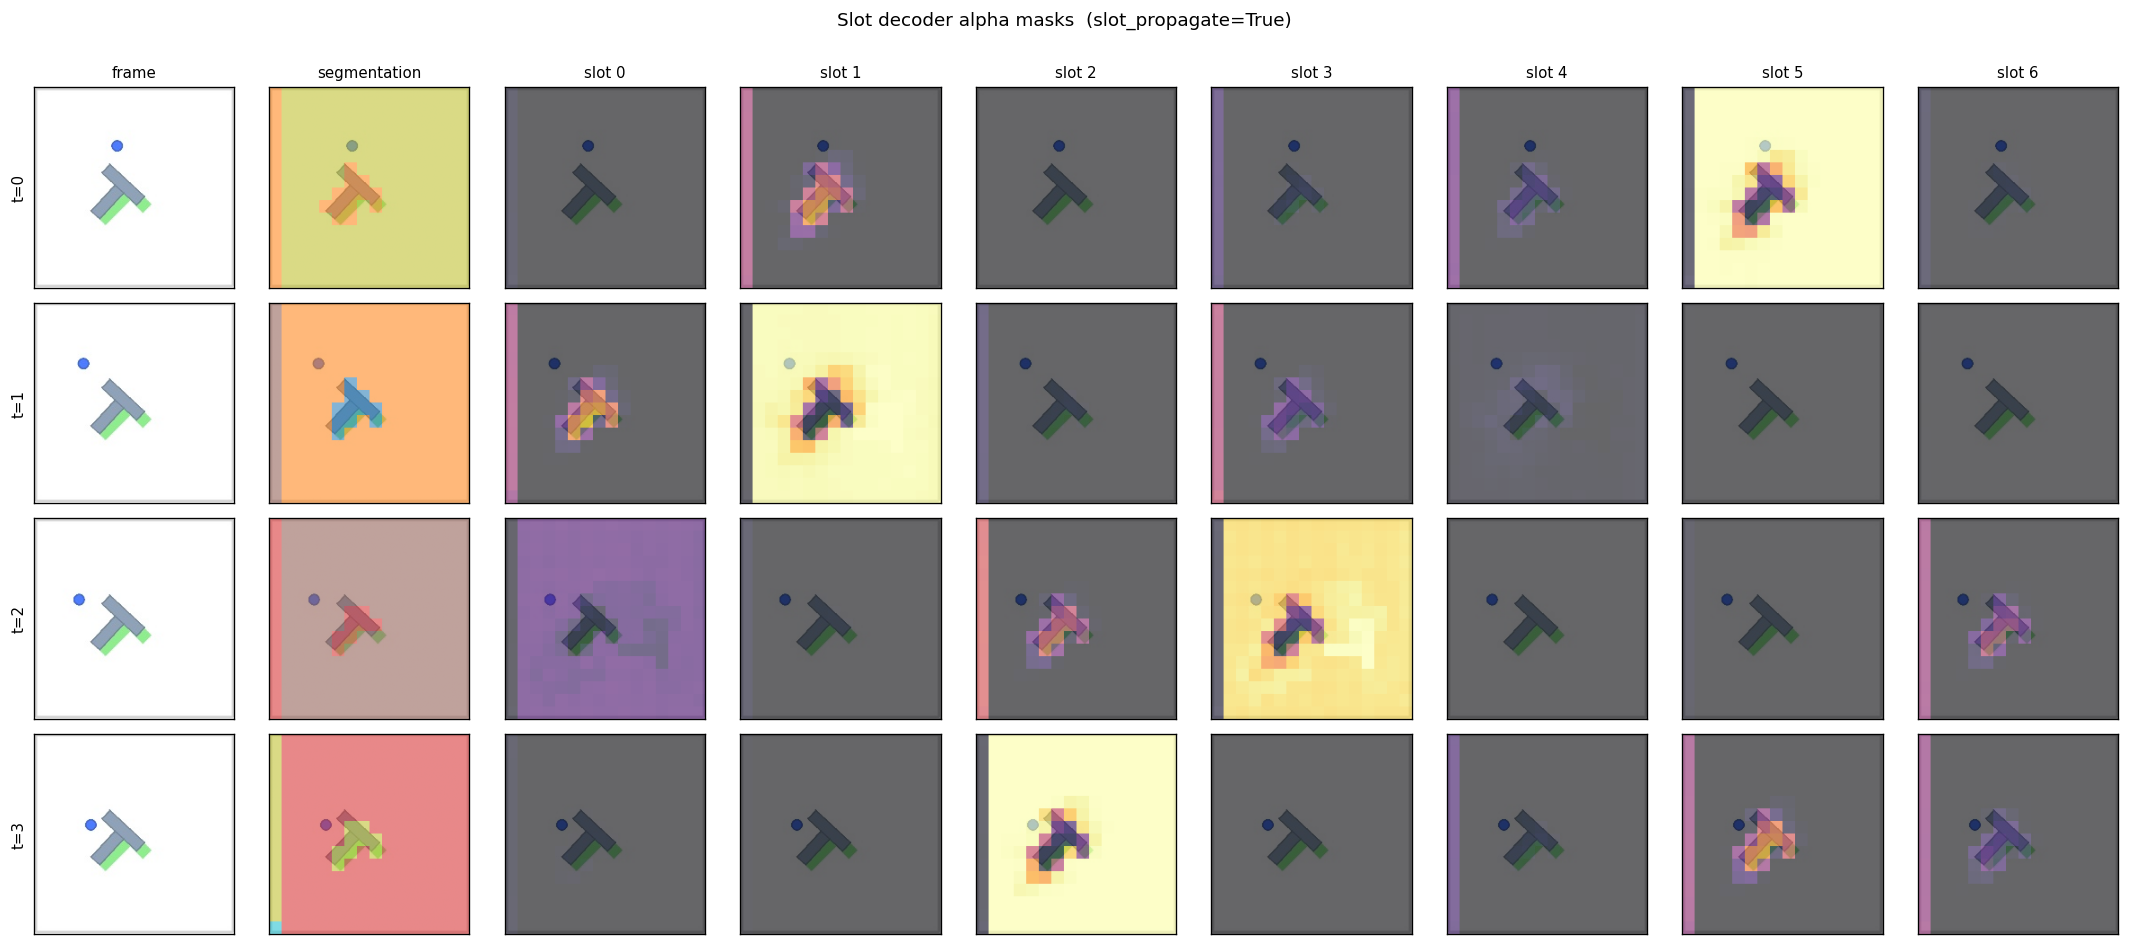
\includegraphics[width=\textwidth]{slots_finetune_0.png}
  \caption{End-to-end finetuned DINOv2 (SAVi on).}
\end{subfigure}\\[0.6em]
\begin{subfigure}{\textwidth}
  \centering
  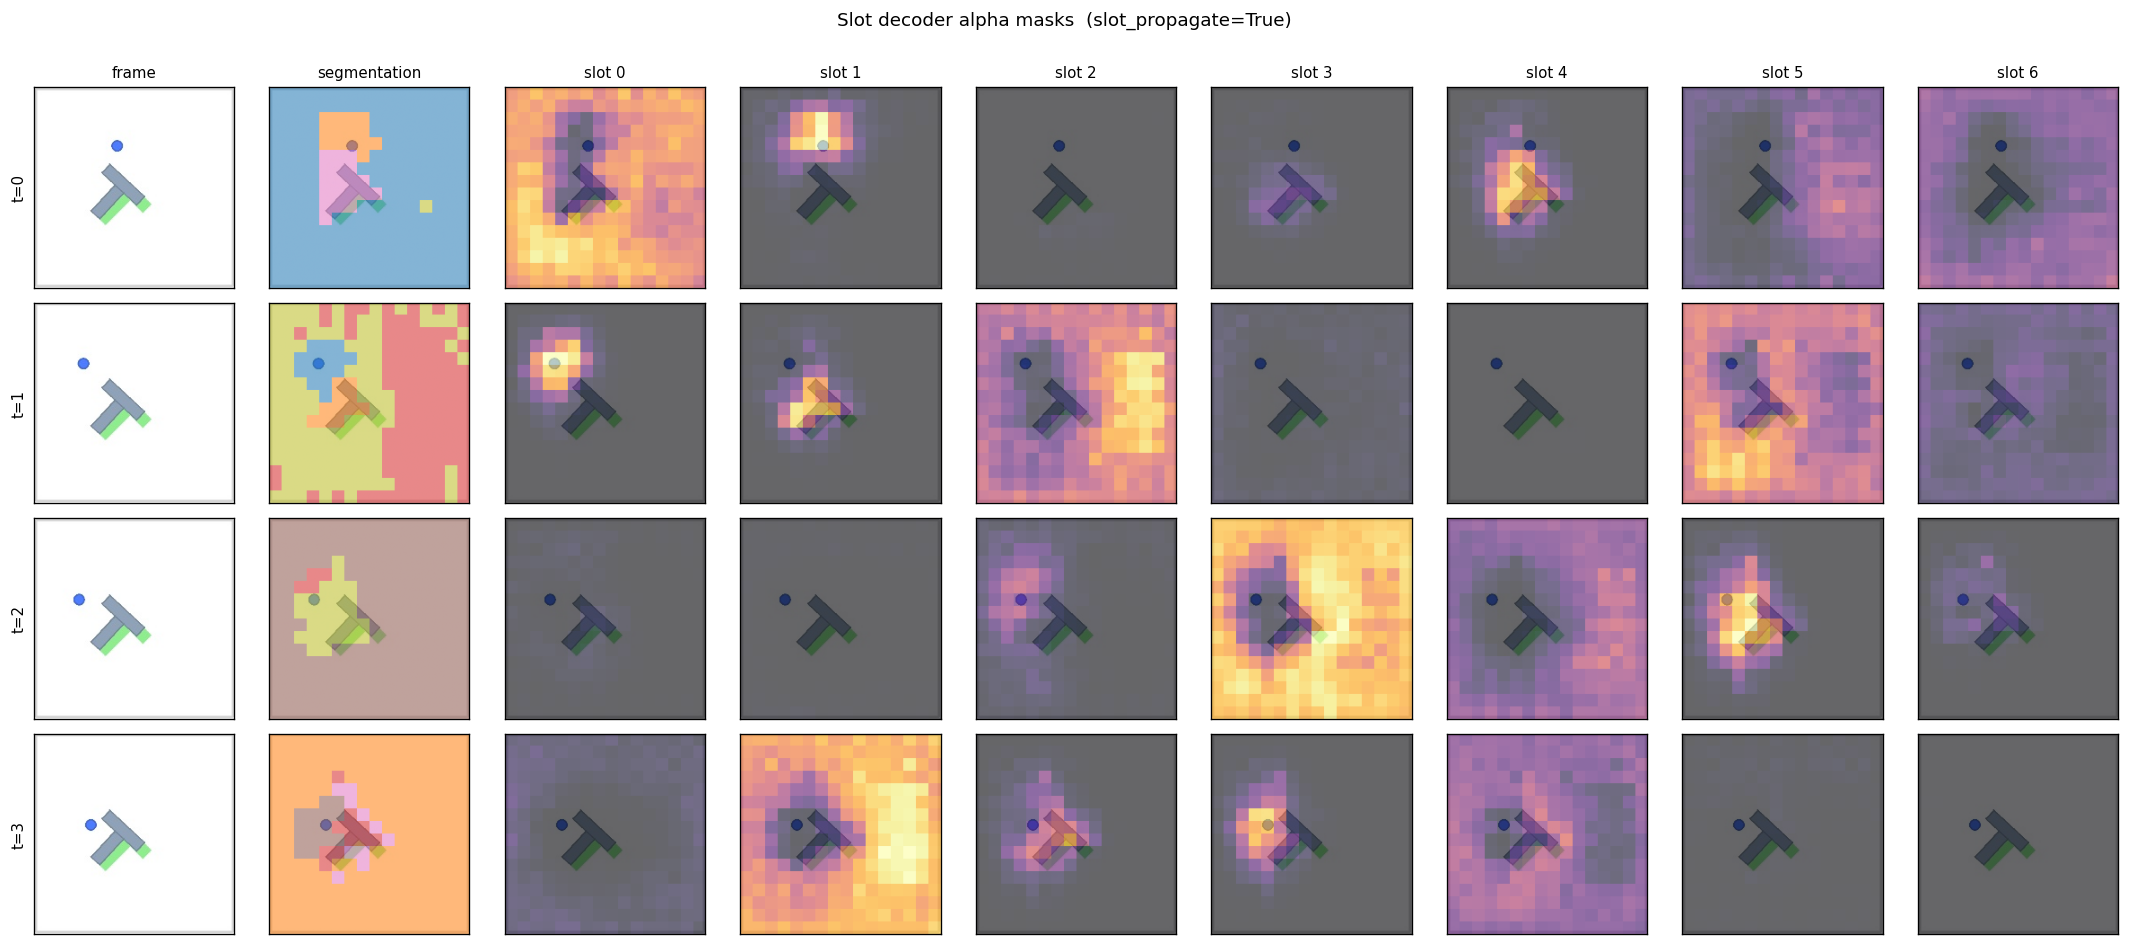
\includegraphics[width=\textwidth]{slots_frozen_0.png}
  \caption{Frozen DINOv2 (SAVi on) --- the quantitative best (Table~\ref{tab:savi}).}
\end{subfigure}\\[0.6em]
\begin{subfigure}{\textwidth}
  \centering
  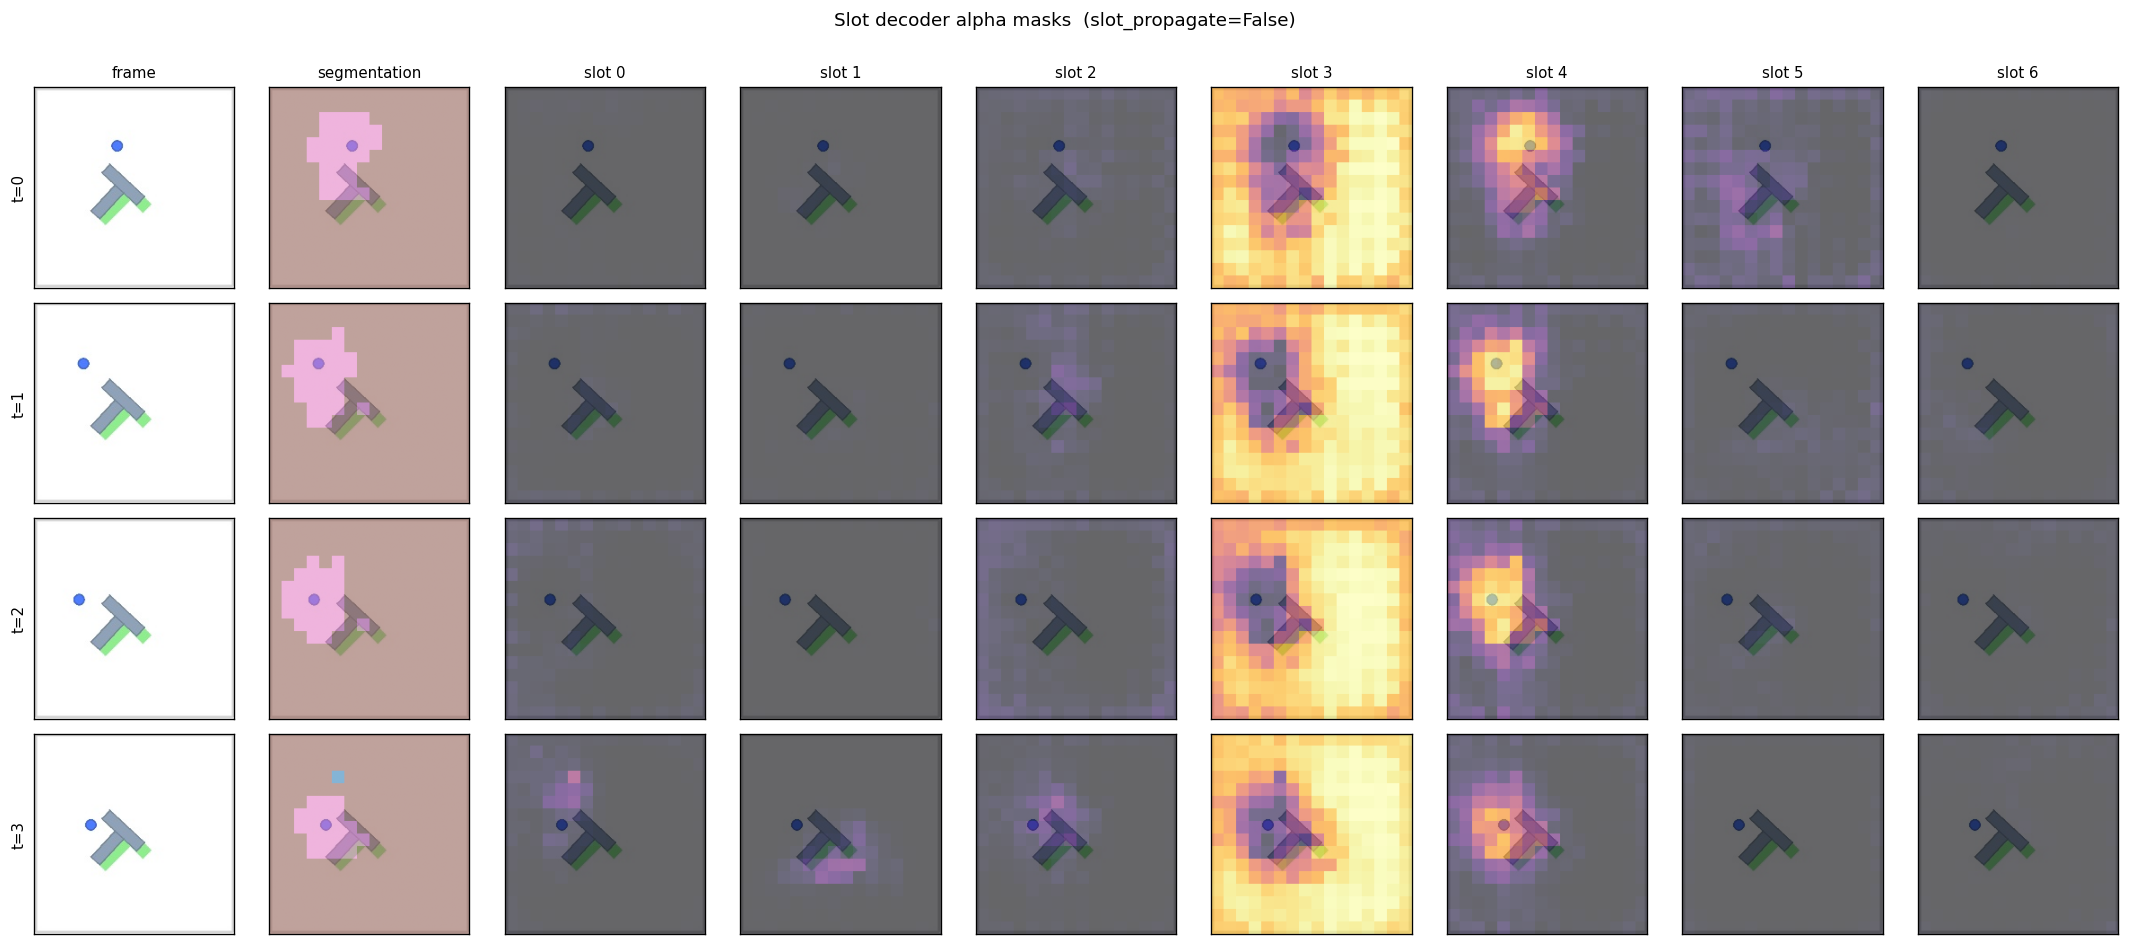
\includegraphics[width=\textwidth]{slots_savioff_0.png}
  \caption{Frozen DINOv2, slot propagation \emph{off}.}
\end{subfigure}
\caption{Decoder alpha masks and argmax segmentation for the same Push-T window ($T{=}4$ rows; columns: frame, segmentation, then the 7 per-slot masks), for the three seed-0 models. Binding crispness ranks finetuned $>$ frozen-on $>$ off; slot-\emph{index} stability over time ranks in the opposite order (see text). Figures for three further windows are in the repository.}
\label{fig:slots}
\end{figure}

Figure~\ref{fig:slots} renders the broadcast decoder's per-slot alpha masks and argmax segmentation for the same window under the three seed-0 models. Three observations, consistent across all four rendered windows:

\paragraph{Slots bind to objects, not noise.} In both SAVi-on models, one slot forms a compact mask hugging the T-block while another takes the background (uniformly active with a dark hole exactly at the T), and the segmentation separates object from background in every frame. This is the visual counterpart of ``reconstruction low + SU $\approx$ 0'': the slots carry scene content and neither collapse mode is present. The models use $\sim$2--3 of 7 slots actively; the pusher ($\sim$1 patch at $16 \times 16$ feature resolution) is not clearly bound by any slot.

\paragraph{End-to-end finetuning visibly improves binding.} Binding crispness ranks \textbf{finetuned $>$ frozen-on $>$ off}: the end-to-end model produces the most compact, object-hugging masks and the cleanest segmentations; the frozen model's masks are more diffuse and patchy; the propagation-off model's masks are blobby, anchored to large background regions, and its segmentation degrades to speckle in some frames. Notably this ranking \emph{disagrees} with the NMSE ranking (frozen 0.235 $<$ finetuned 0.317): prediction error and binding quality measure different things, and the variant embodying the central hypothesis wins on the one that is visible.

\paragraph{Identity stability and prediction dissociate.} Slot-\emph{index} stability over time is \emph{inverted} across arms: the propagation-off model assigns the same slot index to the same role in every frame (per-frame encoding re-derives slots from the same learned anchors --- a near-deterministic role assignment), while both SAVi-on models show the index owning the T-block hopping between frames. Yet the SAVi-on arm predicts $3.4\times$ better (Table~\ref{tab:savi}). Decoder-visible index--role rigidity is therefore \emph{not} what enables prediction; the propagated slot state evidently maintains the temporal correspondence the predictor needs even while the reconstruction roles shuffle. We state this carefully: the alpha masks expose slot \emph{roles under the decoder}, not the predictive latent alignment itself, so this is evidence of a dissociation, not a mechanism identification.

\subsection{Planning evaluation}
\label{sec:planning}

To measure downstream control utility we built a CEM-MPC evaluation harness (\texttt{scripts/eval\_planning.py}) that mirrors LeWM's protocol exactly for comparability: the same \texttt{stable-worldmodel} Push-T environment and success criterion (block within 20\,px positional and $\pi/9$ angular tolerance of the goal), the same task sampling (episode/start pairs from the expert dataset, goal state 25 steps ahead, 50-step evaluation budget, 50 episodes, fixed seed), and the same CEM budget (300 samples $\times$ 30 iterations, top-10\% elites). The policy encodes a 16-frame history window (stride 5), plans a horizon of 5 model steps in slot space against the encoded goal (Algorithm~\ref{alg:cem}), and executes each planned action for 5 environment steps, matching the frameskip-5 action semantics of training.

\begin{table}[t]
\centering
\caption{Push-T CEM-MPC success rate (50 episodes, seed 42, LeWM-matched protocol). All learned policies sit at the random-action floor: with $n{=}50$, success counts of 0--2 are statistically indistinguishable (the 95\% Wilson intervals all overlap and include 2\%). An expert action-replay oracle (replaying each task's recorded actions) recovers the goal, validating that the environment, success criterion, and goal injection are correct.}
\small
\begin{tabular}{@{}lcc@{}}
\toprule
\textbf{Policy} & \textbf{Success rate} & \textbf{Successes / 50} \\
\midrule
Random actions & 2.0\% & 1 \\
Causal-LeWM, frozen SAVi-on (best predictor) & 0.0\% & 0 \\
Causal-LeWM, SAVi-off ablation & 2--4\% & 1--2 \\
\midrule
Expert action-replay (oracle, harness check) & $\approx$100\% & --- \\
\bottomrule
\end{tabular}
\label{tab:planning}
\end{table}

Table~\ref{tab:planning} reports the result, and it is a clear negative: \textbf{none of the learned policies exceed the random-action floor}, and the strongest predictor (frozen SAVi-on, NMSE $0.235$, $\sim$77\% of slot variance explained) succeeds in $0/50$ episodes. The expert action-replay oracle reaches the goal in essentially every episode --- the environment is deterministic given the initial state and action sequence --- so the floor-level learned scores reflect the \emph{planner and representation}, not a harness fault. We therefore present this not as a tuning shortfall but as a substantive finding about \emph{what slot-prediction quality does and does not buy}.

\paragraph{Prediction quality does not imply control utility.} The gap between Table~\ref{tab:savi} (a $3.4\times$ predictive win from SAVi propagation) and Table~\ref{tab:planning} (all arms at chance) is the point: a representation can be highly predictable in its own latent metric yet useless as a planning cost. We trace this to a specific, architectural mismatch between a \emph{coarse latent-space MSE cost} and a \emph{high-precision} control task, on three fronts:
\begin{enumerate}[leftmargin=*]
    \item \textbf{Cost granularity vs.\ task tolerance.} The CEM cost is MSE between predicted and goal \emph{slots}, whose alpha masks resolve the scene at a $16\times16$ patch grid (\S\ref{sec:qual}). Success requires the T-block within $20$\,px and $\pi/9$\,rad --- finer than a patch. Sub-tolerance pose differences barely move the slot-MSE, so the cost landscape the planner optimizes is nearly flat exactly where precision is needed.
    \item \textbf{Action granularity.} Push-T actions are \emph{relative} pusher displacements (scaled by $100$\,px under PD control). The model is conditioned on one action per frameskip-5 step, and the planner holds each chosen action across the 5 environment steps it represents; the recorded data instead applies five distinct sub-actions over that span. One held relative action drives the pusher in a near-straight line, a poor match to the fine corrective motions Push-T rewards.
    \item \textbf{Under-determined dynamics.} Because a single conditioning action stands in for five executed ones, the learned transition is an average over the unseen intermediate actions --- excellent for \emph{predicting} the blurred 5-step outcome (hence the strong NMSE), but lacking the fine action$\rightarrow$effect sensitivity a controller must exploit.
\end{enumerate}
These are not bugs to be patched but design choices inherited from a prediction-first training recipe. They sharply scope the contribution of this paper --- a stably-trained, collapse-free, object-centric world model with strong latent prediction --- and motivate a concrete next research arc toward control (\S\ref{sec:future}): finer, pose-aware costs and per-step action conditioning so that latent predictive quality can translate into closed-loop competence.

% ── 6. Discussion ───────────────────────────────────────────────────
\section{Discussion}

\subsection{Why the Dual Collapse Problem Matters}

The central technical challenge of Causal-LeWM is the simultaneous risk of two distinct collapse modes, now empirically characterized (\S\ref{sec:collapse}):

\begin{itemize}[leftmargin=*]
    \item \textbf{JEPA (noise) collapse:} Without grounding, the encoder produces decorrelated noise slots that satisfy SIGReg and the variance hinge exactly, while the predictor degenerates to mean-prediction at the variance floor. Signature: SU $\rightarrow$ 0, NMSE $\approx$ 1.
    \item \textbf{Slot (identical) collapse:} Without distinctness pressure, slot attention binds all slots to the same content, making prediction trivially easy and reconstruction achievable through a one-slot autoencoder shortcut. Signature: SU $\rightarrow$ 1, NMSE deceptively low.
\end{itemize}

These collapses are synergistic --- the prediction gradient encourages slot collapse, and slot collapse degenerates the distribution SIGReg acts on --- and their signatures are \emph{opposite}, so no single scalar metric detects both. The practical recipe that emerged: reconstruction for content, SIGReg/variance for marginals, within-frame decorrelation for distinctness, and stable slot identity (learned anchors spatially, SAVi propagation temporally) for a well-posed prediction target. Each ingredient maps to a named failure when removed, which we offer as a debugging taxonomy for future object-centric JEPA training.

A second-order lesson: \textbf{collapse metrics and predictive quality are separable axes.} A fully healthy representation (distinct, grounded, stable) still predicted at only 9\% below the mean floor until temporal identity was fixed. Work on anti-collapse regularization should therefore report normalized prediction metrics alongside health metrics.

\subsection{What does slot propagation actually provide?}

The cleanest result in this paper is also the most mechanistically suggestive. Slot propagation changes nothing about what the slots encode (reconstruction and SU identical across arms) yet changes prediction error by $3.4\times$ --- and it does so \emph{without} making the decoder-visible slot roles temporally rigid; indeed the non-propagated model is more rigid in that sense. This suggests the benefit is best understood not as ``slot $n$ always means the T-block'' but as the propagated slot state forming a continuous latent trajectory the predictor can extrapolate, whereas per-frame re-encoding resamples an arbitrary permutation/configuration each frame. Testing this directly (e.g., by measuring cross-frame slot-assignment consistency in latent space, or by training with an explicit Hungarian-matched prediction loss) is a natural next experiment.

\subsection{Limitations}

\begin{enumerate}[leftmargin=*]
    \item \textbf{No demonstrated control utility yet.} The learned policies plan at the random-action floor (\S\ref{sec:planning}); this paper's contribution is representational (stable, collapse-free, strongly-predictive object-centric training), not yet a control result. We argue the failure is an architectural mismatch between a coarse latent cost and a high-precision task (\S\ref{sec:planning}), with a concrete remedy (\S\ref{sec:future}), but that remains to be shown.
    \item \textbf{End-to-end comparison is confounded.} The end-to-end run is a single seed at batch 16 (memory-bound) versus the frozen arm's three seeds at batch 32, and is visibly unconverged at 5{,}000 steps. A frozen baseline at batch 16, a multi-seed end-to-end sweep, longer training, and a warm-start from a frozen checkpoint (supported via \texttt{init\_from}) are the planned dis-confounders.
    \item \textbf{Single-task scope.} The study targets Push-T only. Scaling to CLEVRER for counterfactual VQA --- where C-JEPA's object-level masking showed its largest gains --- remains future work.
    \item \textbf{Fixed slot count; underused slots.} We use $N{=}7$ slots; the models actively use $\sim$2--3 on Push-T, and the small pusher is not cleanly bound at $16 \times 16$ feature resolution.
    \item \textbf{Reintroduced hyperparameters.} Where LeWM reduced tuning to one weight, our objective adds $\lambda_{\text{dec}}$, $\lambda_{\text{rec}}$, and curriculum parameters. We have not yet measured sensitivity to these (all results use one untuned default setting), nor to the aggressive mask target ($\alpha = 0.4$, which a diagnostic showed accounts for roughly half the prediction difficulty).
    \item \textbf{Computational cost.} End-to-end training is $\sim$8$\times$ slower per step than cached frozen training on our hardware; inference cost is unchanged (planning never touches the decoder, and rollouts run purely in slot space).
\end{enumerate}

\subsection{Future Directions}
\label{sec:future}

The planning result (\S\ref{sec:planning}) makes the next research arc concrete: closing the gap between strong latent prediction and closed-loop control.
\begin{itemize}[leftmargin=*]
    \item \textbf{Pose-aware planning costs.} Replace coarse slot-MSE with a cost that resolves the success tolerance --- e.g.\ decoding block pose from slots and scoring in pose space, or a learned slot-to-state readout --- so the planner sees gradient where precision matters.
    \item \textbf{Per-step action conditioning.} Train and plan at the native action rate (or condition each model step on all sub-actions it spans) so plan-time and train-time action semantics match and the dynamics are no longer averaged over unseen intermediate actions.
    \item \textbf{Warm-started end-to-end training:} initialize from a converged frozen-encoder checkpoint and unfreeze, isolating backbone adaptation on top of working slots.
    \item \textbf{Mechanism studies of propagation:} latent-space slot-correspondence metrics and Hungarian-matched prediction targets (\S6.2).
    \item \textbf{Causal graph extraction:} analyzing predictor attention patterns to recover inter-object influence structure induced by the object-level masking.
    \item \textbf{Scaling:} variable slot counts, richer manipulation environments, and CLEVRER counterfactual evaluation, where C-JEPA's object masking showed its largest gains.
\end{itemize}

% ── 7. Conclusion ───────────────────────────────────────────────────
\section{Conclusion}

We presented Causal-LeWM, the first architecture to combine object-level causal masking (from C-JEPA) with end-to-end JEPA training (from LeWM), and the central result is that \textbf{the dual-collapse problem is solved}. Noise collapse and identical-slot collapse have opposite signatures, and a five-term objective whose components are individually load-bearing escapes both at scale --- a stable, collapse-free, object-centric world model trained end-to-end from pixels, which prior object-centric world models avoided by freezing the encoder. On top of this stable foundation we isolate temporal slot identity as the dominant factor in predictive quality: SAVi-style propagation cuts normalized prediction error $3.4\times$ ($0.790 \pm 0.014 \rightarrow 0.235 \pm 0.030$ over three seeds, no overlap) while leaving reconstruction and slot health untouched, and unfreezing the DINOv2 backbone trains stably while producing the sharpest object binding of any variant.

The downstream planning evaluation is, deliberately, reported as a negative result: our learned policies plan at the random-action floor, and a replay oracle confirms the harness is sound. We read this not as a failure of the world model but as an \emph{architectural limitation of applying a coarse latent-space MSE cost to a high-precision robotic task} --- the slot representation that is so strongly predictable in its own metric is finer-grained than a patch yet coarser than the task's $20$\,px tolerance, and the frameskip-averaged dynamics trade fine action sensitivity for predictive smoothness. Far from undercutting the contribution, this cleanly scopes it: the representation-learning problem at the heart of end-to-end object-centric JEPA is solved here, and the precise, well-understood reasons it does not yet plan --- cost granularity and action conditioning --- define a concrete, motivated research sequence (\S\ref{sec:future}) toward turning a strong latent world model into a competent controller.

% ── Acknowledgments ─────────────────────────────────────────────────
\section*{Acknowledgments}

We thank the authors of C-JEPA and LeWM for releasing their code and pretrained models, which made this implementation possible. The Causal-LeWM codebase, experiment log, and all figures are available at \texttt{github.com/Sudarssan-N/cjepa}.

% ── Bibliography ────────────────────────────────────────────────────
\bibliographystyle{plainnat}
\begin{thebibliography}{99}

\bibitem[Assran et~al.(2023)]{assran2023ijepa}
M.~Assran, Q.~Duval, I.~Misra, P.~Bojanowski, P.~Vincent, M.~Rabbat, Y.~LeCun, and N.~Ballas.
\newblock Self-supervised learning from images with a joint-embedding predictive architecture.
\newblock In \textit{CVPR}, 2023.

\bibitem[Bardes et~al.(2022)]{bardes2022vicreg}
A.~Bardes, J.~Ponce, and Y.~LeCun.
\newblock VICReg: Variance-invariance-covariance regularization for self-supervised learning.
\newblock In \textit{ICLR}, 2022.

\bibitem[Chi et~al.(2023)]{chi2023diffusion}
C.~Chi, S.~Feng, Y.~Du, Z.~Xu, E.~Cousineau, B.~Burchfiel, and S.~Song.
\newblock Diffusion policy: Visuomotor policy learning via action diffusion.
\newblock In \textit{RSS}, 2023.

\bibitem[Hafner et~al.(2023)]{hafner2023dreamerv3}
D.~Hafner, J.~Pasukonis, J.~Ba, and T.~Lillicrap.
\newblock Mastering diverse domains through world models.
\newblock \textit{arXiv:2301.04104}, 2023.

\bibitem[Hansen et~al.(2022)]{hansen2022tdmpc}
N.~Hansen, X.~Wang, and H.~Su.
\newblock Temporal difference learning for model predictive control.
\newblock In \textit{ICML}, 2022.

\bibitem[Kipf et~al.(2022)]{kipf2021savi}
T.~Kipf, G.~F.~Elsayed, A.~Mahendran, A.~Stone, S.~Sabour, G.~Heigold, R.~Jonschkowski, A.~Dosovitskiy, and K.~Greff.
\newblock Conditional object-centric learning from video.
\newblock In \textit{ICLR}, 2022.

\bibitem[LeCun(2022)]{lecun2022}
Y.~LeCun.
\newblock A path towards autonomous machine intelligence.
\newblock \textit{OpenReview}, 2022.

\bibitem[Locatello et~al.(2020)]{locatello2020slot}
F.~Locatello, D.~Weissenborn, T.~Unterthiner, A.~Mahendran, G.~Heigold, J.~Uszkoreit, A.~Dosovitskiy, and T.~Kipf.
\newblock Object-centric learning with slot attention.
\newblock In \textit{NeurIPS}, 2020.

\bibitem[Maes et~al.(2026)]{maes2026lewm}
L.~Maes, Q.~Le~Lidec, D.~Scieur, Y.~LeCun, and R.~Balestriero.
\newblock LeWorldModel: Stable end-to-end joint-embedding predictive architecture from pixels.
\newblock \textit{arXiv:2603.19312}, 2026.

\bibitem[Nam et~al.(2026)]{nam2026cjepa}
H.~Nam, Q.~Le~Lidec, L.~Maes, Y.~LeCun, and R.~Balestriero.
\newblock Causal-JEPA: Learning world models through object-level latent interventions.
\newblock \textit{arXiv:2602.11389}, 2026.

\bibitem[Oquab et~al.(2023)]{oquab2023dinov2}
M.~Oquab, T.~Darcet, T.~Moutakanni, H.~Vo, M.~Szafraniec, V.~Khalidov, P.~Fernandez, D.~Haziza, F.~Massa, A.~El-Nouby, et~al.
\newblock DINOv2: Learning robust visual features without supervision.
\newblock \textit{arXiv:2304.07193}, 2023.

\bibitem[Peebles \& Xie(2023)]{peebles2023dit}
W.~Peebles and S.~Xie.
\newblock Scalable diffusion models with transformers.
\newblock In \textit{ICCV}, 2023.

\bibitem[Rubinstein \& Kroese(2004)]{rubinstein2004cem}
R.~Y.~Rubinstein and D.~P.~Kroese.
\newblock \textit{The Cross-Entropy Method: A Unified Approach to Combinatorial Optimization, Monte-Carlo Simulation, and Machine Learning}.
\newblock Springer, 2004.

\bibitem[Seitzer et~al.(2023)]{seitzer2023dinosaur}
M.~Seitzer, M.~Horn, A.~Zadaianchuk, D.~Zietlow, T.~Xiao, C.-J.~Simon-Gabriel, T.~He, Z.~Zhang, B.~Sch\"olkopf, T.~Brox, and F.~Locatello.
\newblock Bridging the gap to real-world object-centric learning.
\newblock In \textit{ICLR}, 2023.

\bibitem[Villar-Corrales et~al.(2022)]{villarcorrales2022ocvp}
A.~Villar-Corrales, S.~Wahdan, and S.~Behnke.
\newblock Object-centric video prediction via decoupling of object dynamics and interactions.
\newblock In \textit{ICIP}, 2022.

\bibitem[Wu et~al.(2023)]{wu2023videosaur}
Z.~Wu, N.~Dvornik, K.~Greff, T.~Kipf, and A.~Garg.
\newblock VideoSAUR: Slot attention for video understanding.
\newblock In \textit{NeurIPS}, 2024.

\end{thebibliography}

\end{document}
